% Copyright 2024 Jay Jay Billings. Some rights reserved.
\documentclass{article}
\usepackage{graphicx} % Required for inserting images
\usepackage{hyperref}
\usepackage{tabularx}
\usepackage{dirtytalk}

\title{Outliving your mind, part 3: No Rocking Chair}
\author{Jay Jay Billings, Ph.D.}
\date{\today}

%In this post, I'll talk about ways families can get help to support their loved ones, including public and private organizations, social support services, legal support for elder care, how and when to engage law enforcement, and how to have tough conversations with family members.

\begin{document}

\maketitle

\begin{center}
\textit{I don't need your rockin' chair, your Geritol or your medicare...}

\hspace*{\fill} - George Jones
\end{center}

\textit{In my \href{https://jayjaybillings.com/2023/07/06/outliving-your-mind-part-1-the-secret/}{last post} on my father's battle with dementia, I shared how his symptoms progressed over time. In this post, I'll talk about how families can get help.}

There's lots of help for families and patients with dementia, and some genuinely skilled medical professionals are dedicated to the practice. The care options cover folks who have simple problems with memory, problems meeting their basic needs, and even the more complicated cases that come with behavioral and psychiatric health concerns. In addition to medical care, there are also numerous government programs and agencies that provide assistance to patients in the U.S. and other countries, laws that support families and protect patients, and aid from social institutions as well. 

Unfortunately, few people prepare for neurological conditions in their golden years. Most people expect death to be quick from a heart attack or drawn out, limiting, and agonizing like cancer. Preparing for this type of end is entirely different than preparing for cognitive decline. This means that dementia can often be like Monty Python's Spanish Inquisition: nobody expects it, and its three weapons are fear, surprise, and ruthless efficiency.

My Dad's case was a good example. He prepared incorrectly because of his lifestyle and not in response to a well-informed understanding of his health (which would have required him to go to the doctor). As I explained in previous posts, he was in superb physical health until his late eighties, and he used this superpower to work, spend time with his children and grandchildren, and fight off people who wanted their money back or the husbands of his mistresses. His great physical health and longevity allowed him to espouse eating a spoonful of Vick's VapoRub (which is not how you use that cream...) as the cure to most illnesses and a good blade, some alcohol, and a bandaid as the best way to tend to a wound. I'm not joking: One time, my little sister called me and asked that I look at some possibly pre-cancerous growths on Dad's head. When I arrived a few hours later, \textit{he handed them to me in a napkin and started cleaning his pocket knife while lecturing me on the need for sterile technique.} 

He adopted the view that he would die suddenly from fisticuffs, a knife, or a bullet. Planning for one's death, in that case, is simple. He saved, bought a burial plot, and left instructions for how he should be interred. But this sudden violent death never came, and he outlived his savings, his friends, his own mind, and even the memories of some of the people with whom he left instructions. To be completely clear about my feelings and absolutely fair to Dad, while he made a poor decision and a bad bet, he still lived well for 93 years! We, his family, hardly tried to convince him otherwise because he seemed to be living a healthy enough life. 

I had many meaningful conversations with Dad about aging, nearly all of which either started or ended with a rousing chorus of George Jones' ``I don't need your rockin' chair.'' While he loved the song, he also lived it. Finding him in an actual rocking chair meant you saw him in a very private moment with only the closest family and friends. This could be like watching Charles Stanley with his children on Sunday after playing in the snow (see figure \ref{fig:rocker}), rocking a grandbaby to sleep, or drinking lemonade on a friend's porch when everyone else had left. He was a proud and old-fashioned man, and he felt that being seen in a rocking chair might give folks the impression that he was old or resting when he shouldn't be. Once the kids, grandkids, and wives were gone, so were our family \href{https://jayjaybillings.com/2016/08/18/family-rocking-chairs}{rocking chairs}, although he kept his recliner. He liked having his legs up while watching the Grand Ole Opry.

In retrospect, there were some \textit{major} mistakes we made as a family that we later had to correct: 
\begin{enumerate}
    \item We never looked at cognitive decline as a serious risk for Dad. This means we never took basic steps that would have improved Dad's care from the start.
    \item We spoke to each other about care plans and preferences too late. This took precious time from us when we needed the information and made everything much more stressful.
    \item I tried to show my wife the health benefits of eating Vick's VapoRub, and now the practice is strictly forbidden in my house. This means I can only rub it on my chest or under my nose, which doesn't seem as effective. (That's a joke: Do not eat Vick's!)
\end{enumerate}

The following sections will describe what we should have done differently when Dad was in good health, including some of the basic steps families can take and the types of organizations that can help.

\begin{figure}[h]
\caption{Proof that Dad would use a rocking chair if it meant he got the space heater to warm his feet after taking us out to play in the snow. Pictured here: me (bottom left), my brother (red hat), and Dad holding my youngest brother in Mom's maroon velvet rocker.}
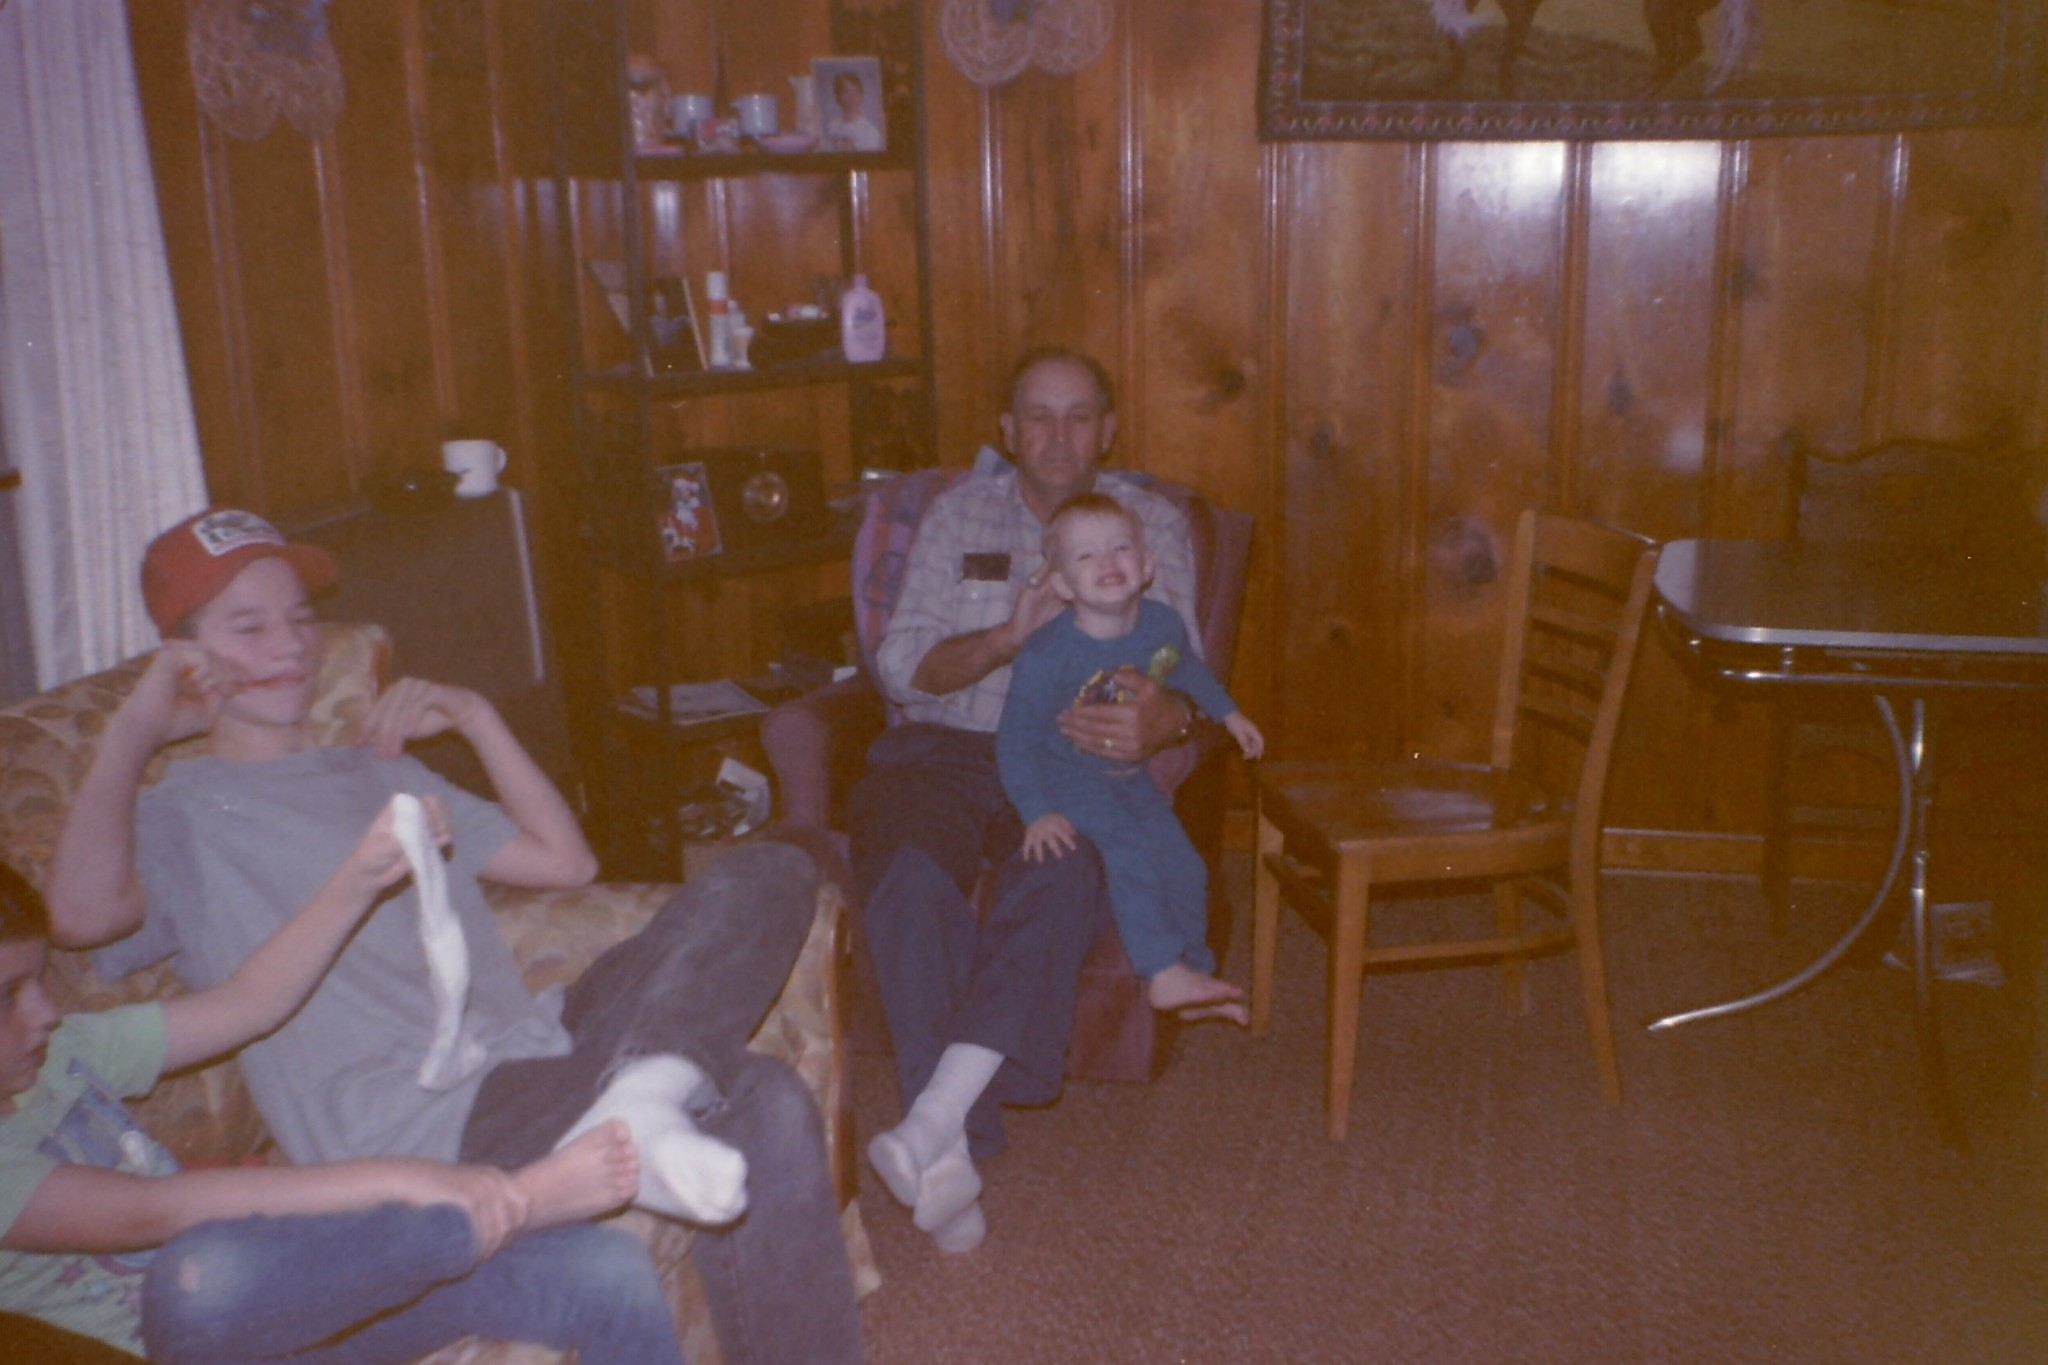
\includegraphics[width=\textwidth]{oym-p3-rocking-chairs/assets/PICT0043.JPG}
\label{fig:rocker}
\end{figure}

\section*{Talking to Family}

My Dad never talked about having a family history of dementia. He said ``something'' about my grandfather getting cranky, which my brother Jack later correctly identified as dementia based on behaviors he remembered too. Dad also told me a story about seeing his grandfather on his deathbed and noted the way he didn't know anyone around him. He just stared at the ceiling. It was only after Dad was experiencing significant cognitive impairment that I found the application for a Civil War pension from his grandmother that described how his grandfather suffered and died. The description was nearly identical to how I would have characterized Dad's experience, and I found it too late to be helpful.

We were short on information and details for almost everything. For example, we knew that Dad wanted to be buried in the family cemetery, but which one and where was it? Once we figured out which one, we had to call our cousins to help find the caretaker to determine how to access the plot.

My siblings and I figured everything out in the end, but only because we could finally communicate and collaborate on the solutions to these unanswered questions. We learned a lesson that is as important as it is a cliche: Communication as a family is the key to success when caring for a disabled loved one. I'm deeply grateful to my siblings for their trust in me and my memory and for the good faith they brought in tough situations.

This brings me to my three tips for talking to family when caring for a loved one as part of a family care team:
\begin{enumerate}
    \item Write down all instructions and preferences that loved ones share about their care and last wishes (i.e., thoughts and plans on long-term care, medical, financial, last rites, burial, etc.) in a notebook that you can share with other caregivers when the time comes. Remember: the best memory is not so firm as faded ink!
    \item When you're having tough conversations with other caregivers, accept that everyone has good intentions, and many, if not all, of the caregivers will have strong and deep feelings about their loved one that encourage them to do the right thing.
    \item Don't be afraid of ``relationship management'' between siblings and caregivers. For example, if it is easier for two particular siblings to talk about an issue than for one sibling to engage everyone, try rolling with it.
\end{enumerate}

Once we got the hang of it, my siblings and I could operate quite efficiently because we recognized that we all loved Dad, wanted to do the right thing, and accepted that sometimes others would speak for us or to us. We became a very effective, distributed team, and we even received several compliments from a judge, lawyers, doctors, nurses, support staff, friends, and other family members on how well we worked together.

It's also helpful to write down how you communicate and work together as a family to save money. If you end up needing a lawyer, they will either thank you for the details or charge you to write them down.

\section*{Legal Support}

Speaking of lawyers...

Aside from talking to friends, loved ones, and personal representatives about what to do should you become incapacitated or die, having the right legal documents or counsel in place is very helpful. If you speak to an attorney (or use a website like Legal Zoom), the most important documents are usually sold as an ``estate planning'' bundle:

\begin{itemize}
    \item A durable power of attorney - This document grants your representative the right to handle your affairs, including your finances and health care decisions.
    \item An advanced medical directive - In the event that you are incapacitated or otherwise unable to communicate your healthcare instructions, this document defines the who, what, when, where, why, and how for your medical needs.
    \item A last will and testament - This document describes what should happen to your estate when you die. Life is a lot easier for your descendants if you have a will, but most people I've met don't have a will or haven't updated their will in a very long time.
\end{itemize}

A ``living will'' is another common estate planning document. It is a type of advanced directive with a narrower scope, and an attorney is the best person to ask if it makes sense to use a living will instead of an advanced medical directive.

These documents make it possible to care for a loved one quickly and without much fuss. For example, the power of attorney and advanced medical directive can be given to healthcare providers to establish the family's rights and the patient's expectations of care, even if they can't discuss it themselves. Everyone should get these documents written when they are young and update them with every significant life change (or at least every decade). However, many people—if not most people—don't. 

Things get very complicated very quickly if these documents don't exist. My father's case required that we petition the court for rights to oversee his medical treatment and finances because he was divorced and did not have any of these documents to establish his wishes. We successfully petitioned the court for two appointments:

\begin{itemize}
    \item Guardianship - This court-appointed role establishes a guardian responsible for all aspects of a person's care except financial decisions. If so granted by the court, it usually includes all medical and day-to-day care decisions.
    \item Conservatorship - This court-appointed role establishes a conservator who is a person's fiduciary and can make financial decisions on their behalf. A conservator cannot make other decisions, including medical decisions. Conservators may be required to post a bond to guarantee the assets they oversee.
\end{itemize}

I skipped over the role of spouses in the discussion above. This is partly out of my own bias since my parents divorced and partly because marriage doesn't universally guarantee the right to support a loved one in a time of need. Only an attorney in your area can tell you exactly what rights a spouse has in your state (or province, country, etc.). Generally speaking, in the United States, a spouse does not have the right to fully manage joint financial assets or to make all medical decisions without a power of attorney. This can get incredibly tricky when someone challenges a spouse's rights or role.

If a separate guardian and conservator are required, they must be able to work together to support their ward (the person for whom they are caring). My brother and I initially considered taking different roles, but there are many advantages to splitting the roles jointly. We decided to be co-guardians and co-conservators since we work very well together and we were also engaging our siblings and other family members.

Guardians and conservators must submit reports to the state after the first six months and every year thereafter. Guardians must report on the health and well-being of their ward, including all changes in health, any procedures performed, and all major changes in their condition. Conservators must report on the ward's finances, including an exact inventory of all the ward's belongings and financial transactions performed on their behalf, their accounts, and any other holdings they may have. On the other hand, an attorney-in-fact (someone acting under a power of attorney) does not have any reporting requirements. Still, it remains a good idea to closely and separately track the same information in case the attorney's decisions are ever contested.

What happens if someone dies without a will? That's a really complicated question that depends on where they lived and where they died. In broad strokes, the survivors (or some interested party if there are no survivors) must present the will to the Clerk of the Court in the appropriate jurisdiction if they had one (called ``dying testate'') or must register as an administrator if the decedent (dead person...) didn't have a will (called ``dying intestate''). Real property passes directly and in equal proportions (in most states) to survivors, and all other assets are managed by the Executor of the will if they died testate or by the Administrator of the Estate if they died intestate. This is another area where only a local attorney can speak for sure because probate law varies widely between jurisdictions.

And that's all I've got to say about that.

\section*{Government Services}

I do not wish to provide an extensive description of government services here; instead, I'll provide only definitions of some of the most common government services. Some of the most important and relevant government services for those suffering from neurological decline are:

\begin{itemize}
    \item Social Security - The Social Security Administration oversees the Old Age, Survivors, and Disability Insurance program, known as Social Security for short. If an applicant is eligible, they can receive a monthly payment from the government to cover their costs of living. More information is available at \url{https://www.ssa.gov/}.
    \item Medicare - Federal health insurance for individuals over 65 years old is provided by the Medicare program. Participants usually have a high opinion of Medicare, which provides high-quality care for most things. My father didn't want the coverage and never registered at 65, so Medicare wanted \$29000 in ``back penalties'' - or \$1000 for every year he didn't use the plan. Unfortunately, we could not use this program with such a hefty fee, so he missed out on extended physical therapy and other treatments.
    \item Medicaid - Impoverished adults and children can seek health benefits from their states through the Medicaid program. Since my father spent everything he had in the later years of his life, this was our only option for his healthcare needs. I believe Medicaid is a fantastic program, and we are deeply grateful for their help and support.
    \item Government Cooperatives - Different public service providers will, in exceptional cases, band together to create cooperatives with staff and resources that are especially suited to helping those in need take advantage of the programs within the covered geographic area. Some of these cooperatives also staff ombudspersons who can support community members; one such ombudsman was invaluable to us.
    \item State Hospitals - Some states provide a network of state-run hospitals for adults with mental and behavioral health issues. Virginia provides nine such hospitals run by the Virginia Department of Behavioral Health and Developmental Services. These hospitals offer high-quality care for patients who may not be able to get it anywhere else due to financial constraints, extreme behavior, or unique medical conditions. State Hospitals are a godsend for patients and families in need of care that can't be obtained anywhere else.
\end{itemize}

\section*{Churches}

There are always churches that will help those in need. The easiest church to contact is your church, and the second easiest is your loved one's church if either of you has such an affiliation. Even if neither of you is religious or a member of a church, many churches still consider it an essential part of their mission to help you.

Some of the most practical services churches provide are ``food trains'' (organized preparation and delivery of meals) and visiting those in long-term care. However, it's the care and love that churches provide to patients and families in their time of need that are the most valuable. Patients can have parishioners visit them if they get lonely, and family members can also have people to talk to. I benefited from my pastor's loving kindness and the hospice chaplain's care and thoughtfulness.

My father also loved the times that ``a beautiful lady from that church'' visited him. He didn't recognize that it was his granddaughter, but he appreciated the attention and discussion!

\section*{Psychiatric Facilities, Long-Term Care, and Home Care}

In all we did to support Dad, I felt we only went against his wishes twice. Of those two things, I think it was the decision to put him in a private long-term care facility that was the hardest on all of us and for which he likely never forgave us. As I discussed in my previous articles, he was also put in the custody of the state hospital twice. This was tougher to handle emotionally because, as we say back home, ``No one wants to go on the Hill'' (even though it is a fantastic facility with an awesome team). However, in both cases, the care provided by these facilities was essential to maintaining a high quality of life.

It is important to point out that it is often a lot harder for families to move someone into a long-term care facility than it is for the patients themselves. Certainly, if that person has only mild cognitive impairment, they may prefer to arrange care in their home, where they still have their cherished belongings and a well-known environment. But what if they have moved in with a loved one that they don't recognize anymore, need medications several times a night, and spend most of their time watching T.V. really loudly because they won't wear hearing aids? Or what if they are very social and living in a long-term care facility provides them the connection to others, activities, and services that they need?

Dementia patients have very particular and special care requirements that vary based on the severity of their symptoms and whether or not there are compounding behavioral health issues. It is important to consider if you and your loved ones are ready to provide constant, twenty-four-hour, seven-day-per-week coverage of someone who is increasingly regressing to the mental state of a toddler in a two-hundred-pound body.

\section*{When to Call the Po-Po}

I wanted to leave the best topic for last; you might say: Sometimes, you have to call the police, and sometimes they might call you.

There are at least four instances where you shouldn't hesitate to involve authorities when caring for your loved ones, even if it feels like you're going to piss some people off. These include:
\begin{itemize}
    \item When someone is threatened
    \item When someone is threatening
    \item When someone is neglected
    \item When someone is hurt
\end{itemize}

As I mentioned \href{https://jayjaybillings.com/2023/07/06/outliving-your-mind-part-1-the-secret/}{in my first article in this series}, the police called us when my father was picked up walking along U.S. Route 11. We also received phone calls from police and hospital staff when my father was sent for ``evaluations'' by one of his long-term care facilities.

We called the police on my father twice. The first was because he was threatening and discharged a pistol at a family member. The second time we called was for his protection when he was being threatened and neglected at a care facility, which invoked his fight response. We worked with authorities to remove him from the facility for his safety and to take him to the hospital, where he could be examined and stabilized. We moved him to a different facility after a short time in the hospital.

What was the final straw that caused him to start fighting? Eight orderlies surrounded him and tried to force him to sit in - of all things - a rocking chair!

\section*{Next Time}

Thanks for reading the third part of my series about my father’s struggles with cognitive decline and what we did to help him. I hope you’ll come back to read the next part, in which I'll discuss what it was like when he died.

I would especially like to thank my wonderful wife Paige for her support, Paige and my friend Brandon Nipper for reviewing my draft, and those who reached out after the earlier articles with kind words of encouragement and gratitude. 

\end{document}
